\chapter{Example chapter}\noindent
This chapter serves as a simple demonstration of what the thesis template looks like.
It provides some simple examples of typical content in academic theses; see \eg \cref{tab:test,fig:test,eq:maxwell}.
In addition, it shows what the default chapters, sections, and margins look like.
For completeness, we also include some references~\cite{feynman,haskell,particle}.

\section{Here is an example section}
Here is an example of a display equation: a self-consistency equation taken from the study of superconductivity.
Note that all equations are left-justified instead of centered. 
In text with a large number of short display equations, this makes the text easier to follow with your eyes, since they don't have to jump large distances at a time.
It also makes the page look more organized due to the constant indentation level.
\begin{equation}
  \Delta(z) = \int_0^{\infty} \!\!\d\epsilon\, \re\!\big[f_s(\epsilon)\big] \tanh\!\left(\frac{\pi}{2e^{\gamma}} \frac{\epsilon/\Delta_0}{T/T_{\textrm{c}}}\right)
\end{equation}
Here is another example, in the form of Maxwell's equations. 
Note the consistent indentation level compared to the equation above.
\begin{equation}
  \begin{aligned}
    \nabla\cdot\symbf{D}  &= \rho, &
    \nabla\times\symbf{E} &= 0 - \partial_{{\kern-0.075em}t{\kern0.04em}}\symbf{B}; \\
    \nabla\cdot\symbf{B}  &= 0, &
    \nabla\times\symbf{H} &= \symbf{J} + \partial_{{\kern-0.075em}t{\kern0.04em}}\symbf{D}. 
  \end{aligned}
  \label{eq:maxwell}
\end{equation}
Finally, we will show some examples of tables and figures.
Note how the width of \cref{tab:test} matches the indentation level of the equations.
The captions are formatted using a small font and extra margins, which helps separate the captions from the surrounding text.
\begin{table}[b!]
  \centering
  \caption{Test table with some mathematical constants.}
  \label{tab:test}
  \begin{tabular*}{\dimexpr\textwidth-4em\relax}{@{\extracolsep{\stretch{1}}\,}lcc@{\,}}
    \toprule
    Name    &   Symbol    &   Value                 \\
    \midrule
    Euler constant          & $e$   & $2.71\ldots$  \\
    Circle constant         & $\pi$ & $3.14\ldots$  \\
    Imaginary identity      & $i$   & $\sqrt{-1}$   \\
    \bottomrule
  \end{tabular*}
\end{table}

\begin{figure}[t!]
  \centering
  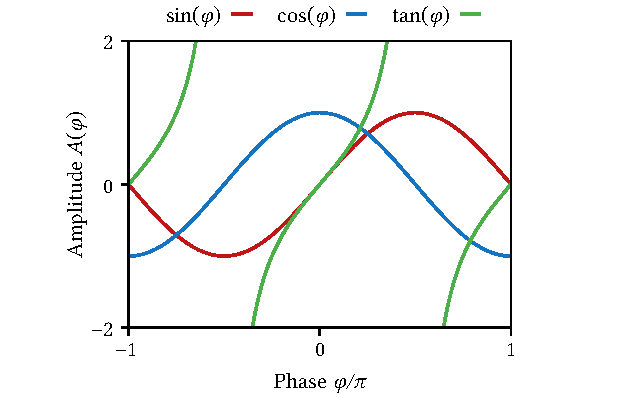
\includegraphics[width=\textwidth]{test.pdf}
  \caption
  {
    This is an example figure made by \textsc{gnuplot}. 
    I have also included an intentionally long caption to show the margins.
  }
  \label{fig:test}
\end{figure}

\section{Lorem ipsum}
\lipsum
